\documentclass[a4paper,12pt]{article}
\usepackage [left=25.4mm,top=25.4mm]{geometry}
\usepackage{amsmath}
\usepackage{amssymb}
\usepackage{graphicx}
%\usepackage{apacite}
\usepackage{url}
\usepackage{subfig}
\usepackage{csvsimple}
\usepackage{float}
\usepackage{lineno}
\usepackage[affil-it]{authblk}
\usepackage{setspace}
\usepackage{makecell} 
\usepackage{tikz}
\usepackage{csvsimple}
\usepackage{newfloat}
\usepackage{xcolor}
\usepackage{tabularx,booktabs}
\usepackage{multirow}
\usepackage{multicol}
\usepackage{array}
\usepackage{tocbasic}
\usepackage{sectsty}

\sectionfont{\fontsize{12}{15}\selectfont}
\chapterfont{\fontsize{14}{15}\selectfont}
\subsectionfont{\fontsize{10}{15}\selectfont}

\newcommand\hcancel[2][black]{\setbox0=\hbox{$#2$}%
	\rlap{\raisebox{.45\ht0}{\textcolor{#1}{\rule{\wd0}{1pt}}}}#2} 
\newcommand{\forceindent}{\leavevmode{\parindent=2em\indent}}

\DeclareFloatingEnvironment[name={Supplementary Figure},fileext=lsf,listname={List of Supplementary Figures}]{suppfigure}
\DeclareFloatingEnvironment[name={Supplementary Table},fileext=lsf,listname={List of Supplementary Tables}]{supptable}
\DeclareFloatingEnvironment[name={Supplementary Material},fileext=lsf,listname={List of Supplementary Material}]{suppmat}

\newcolumntype{P}[1]{>{\centering\arraybackslash}p{#1}}
\newcolumntype{M}[1]{>{\centering\arraybackslash}m{#1}}

\DeclareMathOperator*{\argmax}{arg\,max}
\DeclareMathOperator*{\argmin}{arg\,min}

\newcommand{\indep}{\perp \!\!\! \perp}
\renewcommand*\contentsname{TABLE OF CONTENTS}
\renewcommand{\listfigurename}{LIST OF FIGURES}
\renewcommand{\listtablename}{LIST OF TABLES}

\renewcommand{\arraystretch}{1.5}
\begin{document}
	\begin{titlepage}
		\title{Modularity Examples}
		\author[1]{Jarred M. Kvamme}
		\affil[1]{Department of Bioinformatics and Computational Biology - University of Idaho}
		\maketitle
	\end{titlepage}
	
	
	\newpage
	\tableofcontents
	\addcontentsline{toc}{section}{LIST OF TABLES}
	\addcontentsline{toc}{section}{LIST OF FIGURES}
	\listoftables
	\listoffigures
	\newpage
	
	\section{Background}
	A common goal in network inference is to identify communities of nodes based on their network structure. A community is therefore a subnetwork in which nodes in the sub-network are more densely connected than nodes outside of the network. Modularity is a quantitative metric commonly employed \cite{} to assess the quality of a network partition relative to the network structure. The total modularity for a partition of a network into $k$ communities/sub-networks is given by
	
	\[Q = \sum_{k=1}^K\frac{\Sigma_{in,k}}{2m} - \left(\frac{\Sigma_{tot,k}}{2m}\right)^2 \]
	
	\noindent where $\Sigma_{in,k}$ is the total number of edges within the $k^{th}$ community, $\Sigma_{tot,k}$ is the total number of edges incident to each node in community $k$ (i.e their total degree), and $m$ is the number of edges in the network. 
	\\
	
	The first term $\frac{\Sigma_{in,k}}{2m}$ represents the fraction of edges in the network that lie within sub-community $k$ and second term $\left(\frac{\Sigma_{tot,k}}{2m}\right)^2$ is the expected fraction of edges for a random graph with the same degree distribution. Therefore, this metric represents the degree to which the observed partition deviates from the null model under the random graph. The modularity values between -1 and 1, however, the actual maximum value is dependent on the size of the network \cite{}. Values greater than 0 indicate higher quality partitions and can be interpreted as a higher than expected density of edges constituting potential community structure. In the following report we outline several simple examples of using modularity as a quality function for a network partition in order to characterize its overall behavior and the influences of network structure. 
	
	\section{Case 1: Two completely disconnected communities}
	In this first case, we explore how modularity is influenced by community structure exploring an elementary example consisting of two completely disconnected ring-like sub-networks of $5$ nodes each. These two sub-networks correspond to two communities. We focus on two examples: \textbf{Example 1} consists of calculating the modularity when the nodes in sub-networks assigned to their correct communities and \textbf{Example 2} consists of calculating the modularity when all the nodes are assigned to a single community \textbf{Figure \ref{fig:case1}}.
	\begin{figure}[H]
		\centering
		\caption{Case 1 graph}
		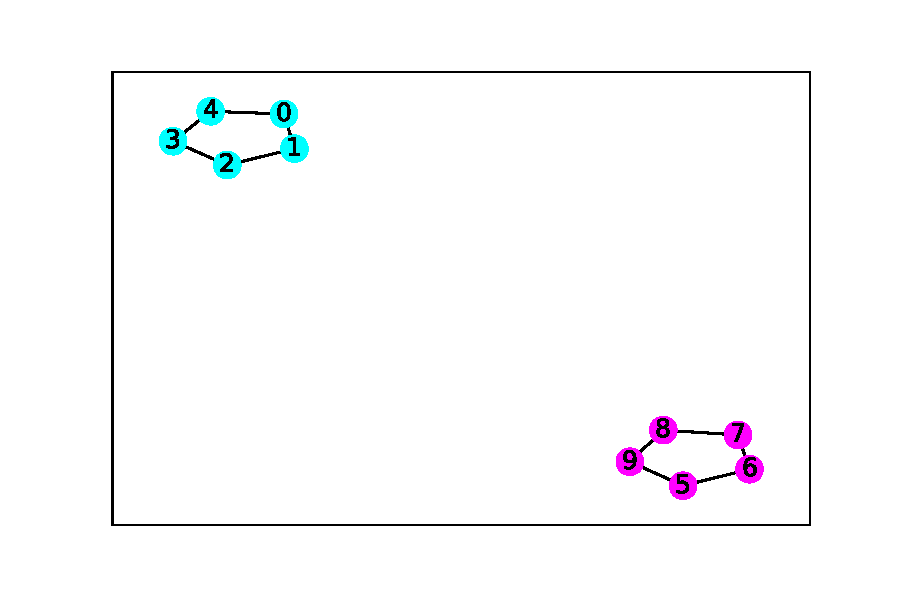
\includegraphics[scale=0.65]{C:/Users/Bruin/Documents/GitHub/HGRN_repo/Modularity/case1_2clusts.pdf}
		\label{fig:case1}
	\end{figure}
	\subsection{Example 1: Modularity for two communities of 5 nodes}
	We start by computing the modularity for community one (teal). The structure of each sub-network is identical which greatly simplified the calculations. For community 1, the number of edges within is $\Sigma_{in,1} = 2\times5$, the number of incident edges is $\Sigma_{tot,1} = 10$ and $m = 10$. Therefore the modularity of community 1 is 
	\[Q_1 = \frac{10}{2(10)} - \frac{10^2}{4(100)} = 0.25\]
	similarly for community 2 we have 
	\[Q_2 = \frac{10}{2(10)} - \frac{10^2}{4(100)} = 0.25\]
	Therefore the total modularity is the sum of the modularity of each community:
	
	\[ Q = \sum_{k=1}^2 Q_k = 0.5\]
	\subsection{Example 2: Modularity for a single community of 10 nodes}
	In our second example we compute the modularity when all of the nodes are grouped into a single community. The is gives $\Sigma_{in,1} = 2(10) = 20$, $\Sigma_{tot,1} = 2(10) = 20$,  $m = 10$ which gives:
	
	\[ Q = \frac{20}{2(10)}-\frac{20^2}{4(100)} = 1-1 = 0 \]
	
	

	\section{Case 2: A single ring-network divided into 2 communities}
	In this second case, we explore how modularity is influenced by community structure through another elementary example in which we have a single ring-structured community which is divided evenly into two sub-networks of $5$ nodes each \textbf{\textbf{Figure \ref{fig:case2}}}. We again focus on two examples: \textbf{Example 1} calculating the modularity when the nodes are divided into two communities and \textbf{Example 2} calculating the modularity when all the nodes in the ring are assigned to a single community. 
	\begin{figure}[H]
		\centering
		\caption{Case 2 graph}
		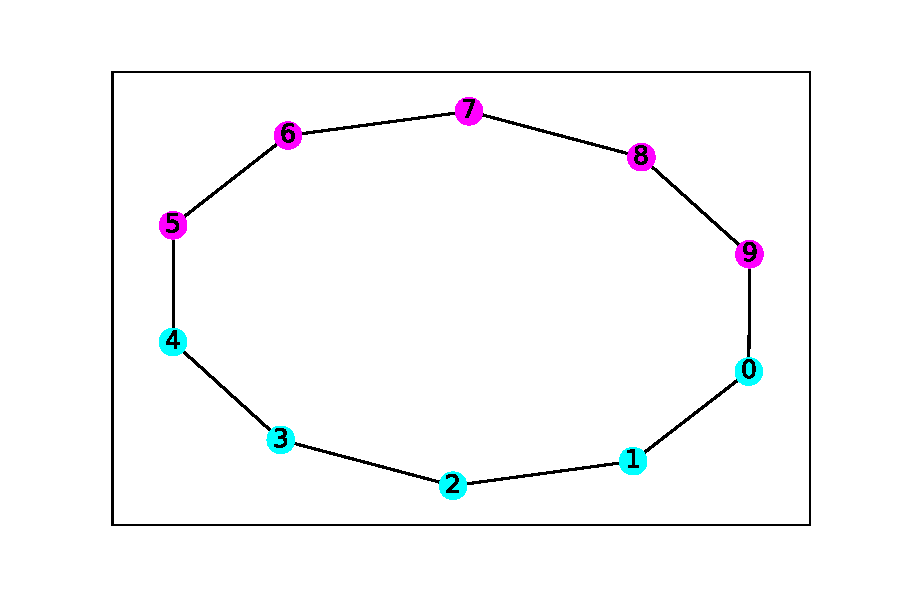
\includegraphics[scale=0.65]{C:/Users/Bruin/Documents/GitHub/HGRN_repo/Modularity/on_net_multi_comms.pdf}
		\label{fig:case2}
	\end{figure}
	
	
	\subsection{Example 1: Modularity for a ring divided into two communities of 5 nodes}
		We start by computing the individual modularities for each community. Again structure of each sub-network is identical making the calculations simple. For community 1, the number of edges within is $\Sigma_{in,1} = 2\times4$, the number of incident edges is $\Sigma_{tot,1} = 10$ and $m = 10$. Therefore the modularity of community 1 is 
		\[Q_1 = \frac{8}{2(10)} - \frac{10^2}{4(20)} = 0.15\]
		similarly for community 2 we have 
		\[Q_2 = \frac{10}{2(20)} - \frac{10^2}{4(20)} = 0.15\]
		Therefore the total modularity is the sum of the modularity of each community:
	
	\[ Q = \sum_{k=1}^2 Q_k = 0.3\]
	\newpage
	\subsection{Example 2: Modularity for all nodes in a single community}
		In our second example we compute the modularity when all of the nodes are grouped into a single community. The is gives $\Sigma_{in,1} = 2(10) = 20$, $\Sigma_{tot,1} = 2(10) = 20$,  $m = 10$ which gives:
	
		\[ Q = \frac{20}{2(10)}-\frac{20^2}{4(100)} = 1-1 = 0 \]
	
	
	
	
	
	
	
	
	
	
	
	
	
	
	
	
	
	
	
	
	
	

	\section{Case 3: The case of a singleton community}
	In this second example, we explore how modularity is affected by the presence of a singleton community \textbf{Figure \ref{fig:case3}}. In \textbf{Example 1} we calculate the modularity when there are two communities where one community consists of a single isolated node (singleton) and the other community consists of a community of 5 nodes. In \textbf{Example 2} we expand on \textbf{Example 1} by allowing the singleton community to have a single edge connecting it the primary network of 5 nodes \textbf{Figure \ref{fig:case3b}}. Lastly, in \textbf{Examples 3-4} we calculate the modularity for \textbf{Examples 1-2} when grouping all nodes into a single community. 
	
	\begin{figure}[H]
		\centering
		\caption{Case 3 graph}
		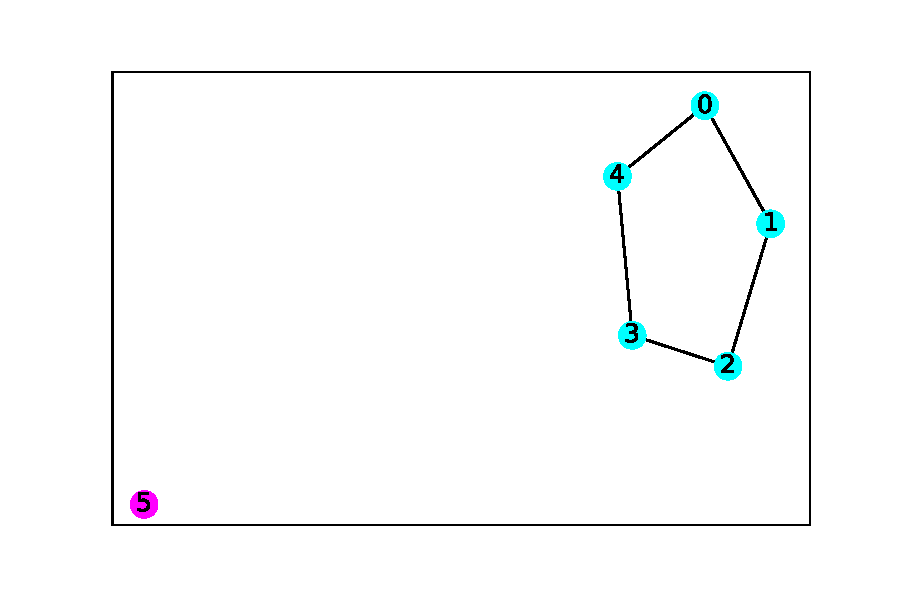
\includegraphics[scale=0.65]{C:/Users/Bruin/Documents/GitHub/HGRN_repo/Modularity/case2_singleton.pdf}
		\label{fig:case3}
	\end{figure}
	
	\subsection{Example 1: Modularity for a ring divided into two communities of 5 nodes}
	We start by computing the individual modularities for each community. For the singleton community, the number of edges within is $\Sigma_{in,1} = 0$, the number of incident edges is $\Sigma_{tot,1} = 5$ and $m = 5$. Therefore the modularity of the singleton community is 
	\[Q_1 = \frac{0}{2(5)} - \frac{0^2}{4(25)} = 0\]
	For the second community of five nodes in a ring structure, we have 
	\[Q_2 = \frac{10}{2(5)} - \frac{10^2}{4(25)} = 0\]
	Therefore the total modularity is the sum of the modularity of each community:
	
	\[ Q = \sum_{k=1}^K Q_k = 0\]
	\subsection{Example 2: Modularity for all nodes in a single community}
	In our second example we compute the modularity similar to \textbf{Example 1} but now the singleton community share a single edge to the other community of give nodes. The choice of which node the edge connects to is arbitrary and does not effect the modularity.  
	
	\begin{figure}[H]
		\centering
		\caption{Case 3(b) graph}
		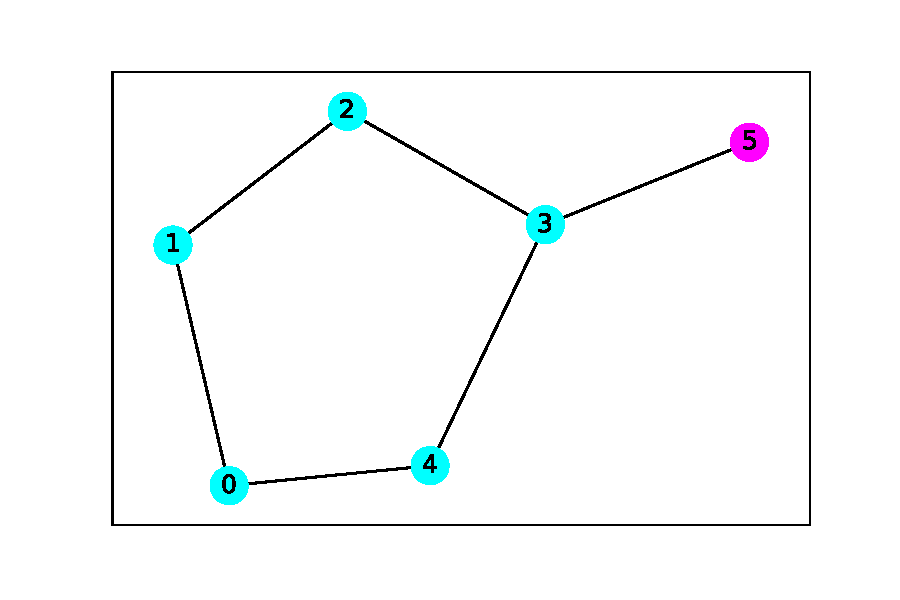
\includegraphics[scale=0.65]{C:/Users/Bruin/Documents/GitHub/HGRN_repo/Modularity/singleton_with_edge.pdf}
		\label{fig:case3b}
	\end{figure}
	
	For the singleton community, the number of edges within is still $\Sigma_{in,1} = 0$, the number of incident edges is now $\Sigma_{tot,1} = 6$ and $m = 6$. Therefore the modularity of the singleton community is 
	\[Q_1 = \frac{0}{2(6)} - \frac{1^2}{4(36)} = -0.00694\]
	The same value as before. For the second community of five nodes in a ring structure, we have 
	\[Q_2 = \frac{10}{2(6)} - \frac{11^2}{4(100)} = -0.00694\]
	Therefore the total modularity is the sum of the modularity of each community:
	
	\[ Q = \sum_{k=1}^K Q_k = -0.01389\]
	
	\subsection{Example 3: Example 1 with a single community}
	In this third example we compute the modularity when all of the nodes from the graph in \textbf{Example 1} are grouped into a single community. The is gives $\Sigma_{in} = 2(5) = 10$, $\Sigma_{tot} = 2(5) = 10$,  $m = 5$ which gives:
	
	\[ Q = \frac{10}{2(5)}-\frac{10^2}{4(25)} = 1-1 = 0 \]
	\subsection{Example 4: Example 2 with a single community}
	Lastly, for the fourth example we compute the modularity when all of the nodes from the graph in \textbf{Example 2} are grouped into a single community. The is gives $\Sigma_{in} = 2(6) = 12$, $\Sigma_{tot} = 2(6) = 12$,  $m = 6$ which gives:
	
	\[ Q = \frac{12}{2(6)}-\frac{12^2}{4(36)} = 1-1 = 0 \]
	
	\section{Partitioning 3 communities}
	\subsection{Scenario 1}
	In this example, we investigate the impact of modularity on network partitions as the number of edges between communities changes. We model three communities with varying sizes denoted as $n_1, n_2, n_3$ and having degree $d$. Initially, the communities are isolated, containing only internal edges. Our exploration begins with a straightforward case, referred to as \textbf{Scenario 1}. Here, we set $n_1 = n_2 = n_3 = 3$ and $d = 2$ for all communities. Subsequently, we analyze how modularity differs between a two-community and a three-community partition as edges are introduced between communities 1 and 2 (refer to \ref{fig:add_case1_simplots}).
	\subsection{Scenario 2}
	In the more complex \textbf{Scenario 2}, we expand upon the previous scenario by considering larger communities with varying node counts: $n_1 = 20, n_2 = 15, n_3 = 10$ with $d = 2$ (refer to \ref{fig:add_sim2_simplots}). In both scenarios, our observations reveal that modularity initially supports the finer three-community partition. This trend persists until a crucial inflection point, where the preference shifts towards a two-community partition. At this inflection point, community 1 and community 2 merge into a single community. Notably, this transition consistently occurs when the number of edges between communities 1 and 2 surpasses the maximum number of internal edges within any of the communities. This finding suggests a critical threshold, beyond which the network structure favors a more cohesive two-community arrangement.
	
	\begin{figure}[H]
		\caption{\textbf{Scenario 1} simulation results for comparing modularity of community partitions with 2 and 3 nodes. (\textbf{Top Left}) The orange line represents the total modularity for a partition of the nodes according to the 3 original communities of 3 nodes each. The blue line represents the total modularity for a partition into two communities i.e merging communitities 1 and 2 into a single community. The $x$-axis gives the number of edges between the two merged communities. (\textbf{Top Right}) The starting graph with 3 completely separated communities. (\textbf{Bottom Left}) the individual modularities for each community as the number of edges between communities 1 and 2 are increased. (\textbf{Bottom Right}) The difference in total modularity for partitions of 2 and 3 communities as a function of the number of edges between communities 1 and 2}
		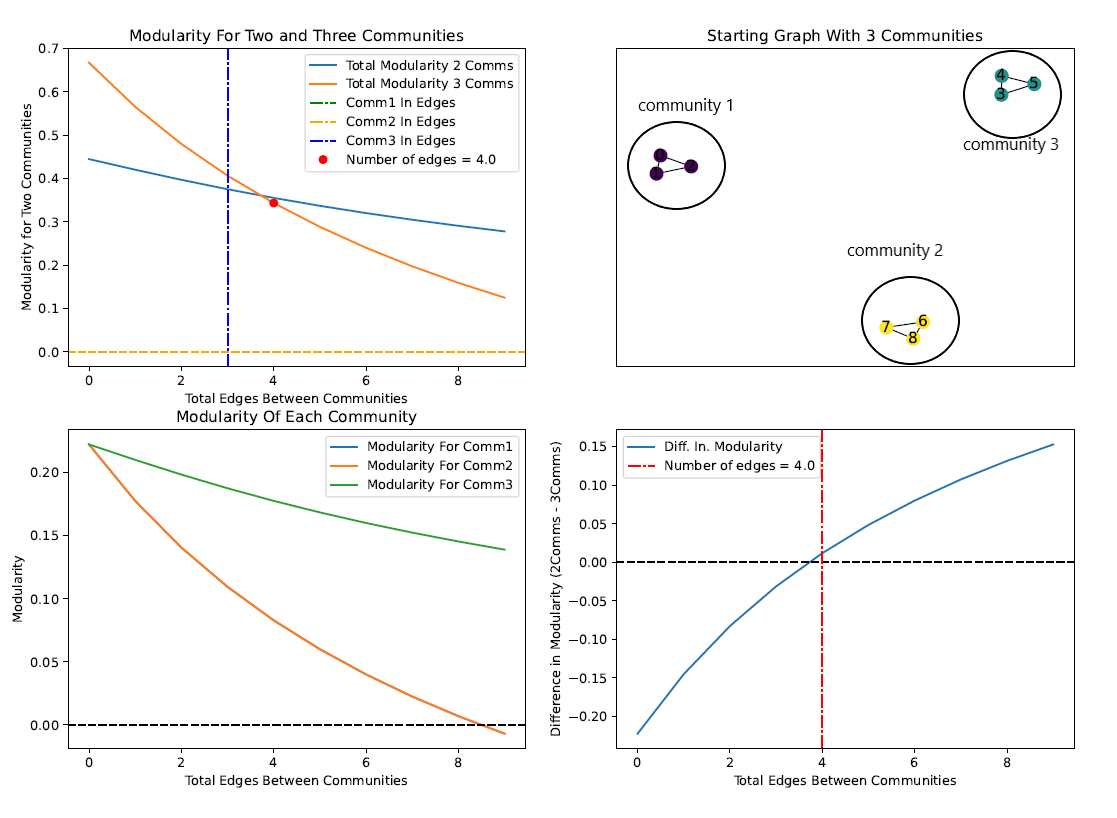
\includegraphics[scale=0.55]{C:/Users/Bruin/Documents/GitHub/HGRN_repo/Modularity/simplest_case_3community_iteradd_sim_plots.png}
		\label{fig:add_case1_simplots}
	\end{figure}
	
	\begin{figure}[H]
		\caption{\textbf{Scenario 2} simulation results for comparing modularity of community partitions with 2 and 3 nodes. (\textbf{Top Left}) The orange line represents the total modularity for a partition of the nodes according to the 3 original communities of 3 nodes each. The blue line represents the total modularity for a partition into two communities i.e merging communities 1 and 2 into a single community. The $x$-axis gives the number of edges between the two merged communities. (\textbf{Top Right}) The starting graph with 3 completely separated communities. (\textbf{Bottom Left}) the individual modularity for each community as the number of edges between communities 1 and 2 are increased. (\textbf{Bottom Right}) The difference in total modularity for partitions of 2 and 3 communities as a function of the number of edges between communities 1 and 2}
		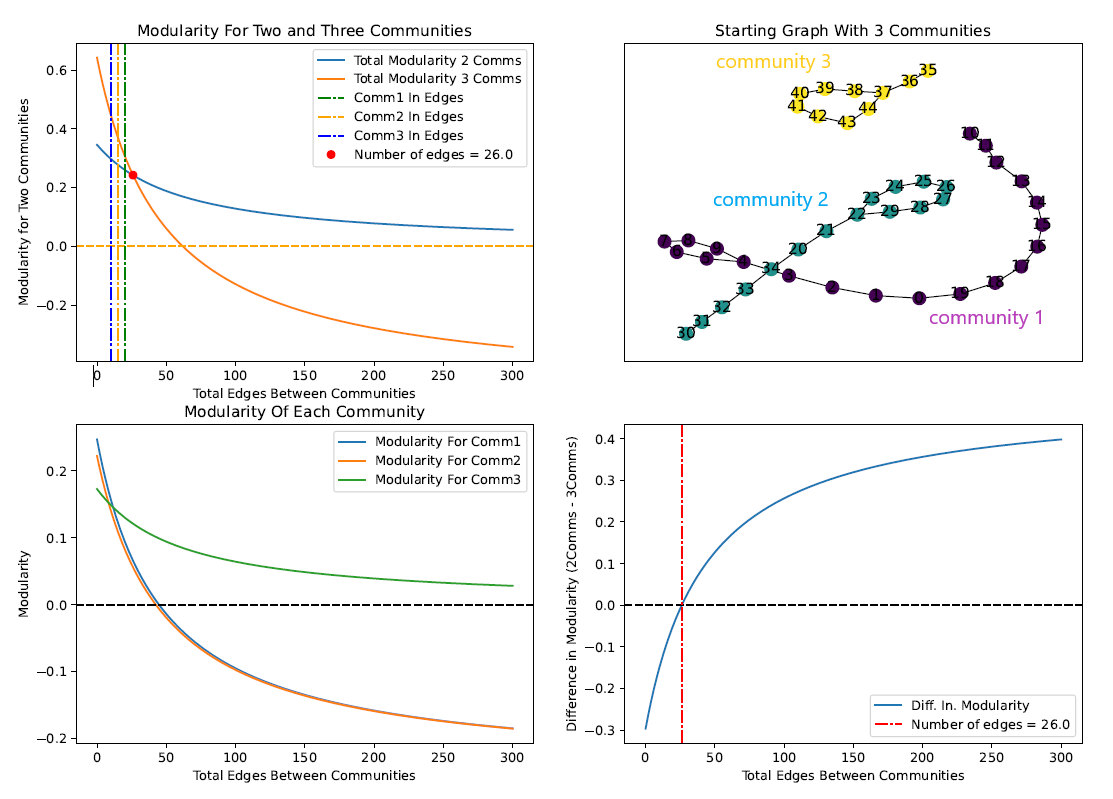
\includegraphics[scale=0.6]{C:/Users/Bruin/Documents/GitHub/HGRN_repo/Modularity/complex_case1_3community_iteradd_sim_plots.png}
		\label{fig:add_sim2_simplots}
	\end{figure}
	
	
	
	\section{Hierarchy Example:}
	
	We now expand our example to incorporate a simple hierarchical structure consisting of three layers, as illustrated in \textbf{Figure \ref{fig:hierarchy_example}}. The top layer of the hierarchy comprises two interconnected nodes. Each of these nodes gives rise to three child nodes, forming communities at the middle layer. Each node in the middle layer possesses two internal edges, and a single edge connects the two communities of three nodes. To gain a deeper insight into how this hierarchical organization correlates with modularity optimization, we calculate the modularity of the communities corresponding to both the middle and top layers of the hierarchy. This analysis is conducted on the graph containing 18 nodes at the observed hierarchical level. Below we give the calculated modularity for a partition of the network into the 6 communities corresponding to the six nodes at the middle level of the hierarchy
	The modularity for communities 1,3,4, and 6
	\[ 4\times \left[\frac{2\times 3}{2\times 25}-\left(\frac{3+3+2}{2\times 25}\right)^2\right] =  4\times \left[\frac{6}{50}-\left(\frac{8}{50}\right)^2\right] = 4\times 0.0944 = 0.3776\]
	
	Modularity for communities 2 and 5
	\[ 2\times \left[\frac{2\times 3}{2\times 25}-\left(\frac{3+3+3}{2\times 25}\right)^2\right] =  2\times \left[\frac{6}{50}-\left(\frac{9}{50}\right)^2\right] = 2\times 0.0876 = 0.1752\]
	
	The total modularity is 
	\[M = 0.3776 + 0.1752 = 0.553 \]
	
	The modularity for a partition of the hierarchy into two communities is given by 
	\[ 2\times \left[\frac{2\times 12}{2\times 25}-\left(\frac{2(3+3+3)+(3+3+3)}{2\times 25}\right)^2\right] =  2\times \left[\frac{24}{50}-\left(\frac{25}{50}\right)^2\right] = 2\times 0.229 \approx 0.46\]
	
	In this particular example, it's worth noting that each pair of communities, regardless of whether the network is partitioned into six nodes or the two nodes at the top level, shares only a single edge between them. This structural characteristic aligns with our earlier observations in both \textbf{Scenarios 1 and 2}. Specifically, we find that the partition corresponding to the six nodes in the middle layer of the hierarchy achieves a slightly higher modularity score compared to the partition based on the top layer nodes. The reason for this distinction lies in the higher within-community edge density of the finer partition. In contrast, the partition into two communities results in a "less than expected" or sparser configuration within the communities, reducing the overall modularity score.
	
	\begin{figure}[H]
		\caption{\textbf{Hierarchy Example} A simple hierarchy example for modularity with a top layer composed of two super level communities, 6 middle level communities and $n = 18$ nodes at the bottom (observed) level of the hierarchy. \textbf{A.)} A side profile of the hierarchy. \textbf{B.)} A "top-down" view of the hierarchy}
		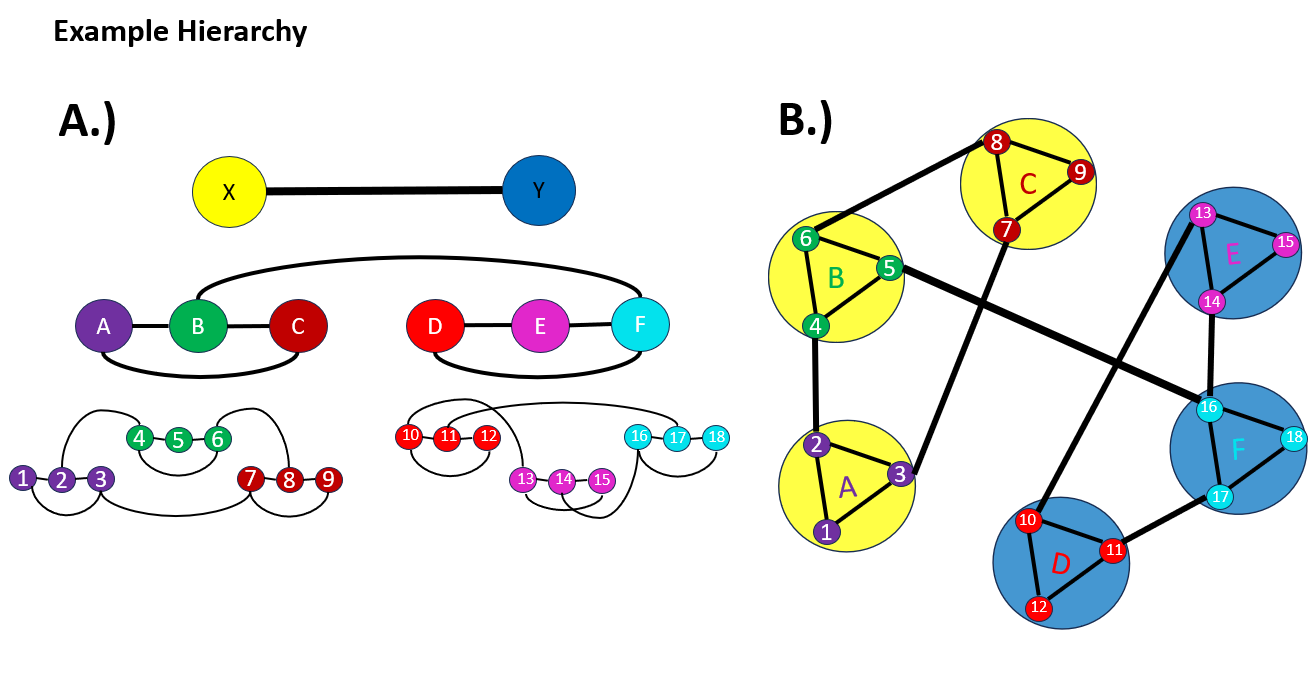
\includegraphics[scale=0.5]{C:/Users/Bruin/Documents/GitHub/HGRN_repo/Modularity/Hierarchy_Example_fig.png}
		\label{fig:hierarchy_example}
	\end{figure}
	
	\section{Conclusions}
	
	
	
	
	
	
	
	
	
	
	
	
	
	
	
	
	
	
	
	
	
	
	
	
	
	
	
	
	
	
	
	
	
	
	
	
	
	
	
	
	
	\newpage
	\appendix
	
	\section*{Case 1 In Linear Form}
	Please refer to the network in \textbf{Figure \ref{fig:case1}}:
	
	\subsection*{Example 1: Modularity for two communities of 5 nodes}
	Let $\bf{C}$ be the the community assignment matrix 
	\[ {\bf C} = \begin{bmatrix}1 & 0 \\ 1 & 0 \\ 1 & 0 \\ 1 & 0 \\ 1 & 0 \\ 1 & 0 \\ 0 & 1 \\ 0 & 1 \\ 0 & 1 \\ 0 & 1 \\ 0 & 1 \\
	\end{bmatrix}\] 
	
	Let $\bf A$ be the graph adjacency matrix
	\[ {\bf A} = \begin{bmatrix}
		0& 1& 0& 0& 1& 0& 0& 0& 0& 0\\
		1& 0& 1& 0& 0& 0& 0& 0& 0& 0\\
		0& 1& 0& 1& 0& 0& 0& 0& 0& 0\\
		0& 0& 1& 0& 1& 0& 0& 0& 0& 0\\
		1& 0& 0& 1& 0& 0& 0& 0& 0& 0\\
		0& 0& 0& 0& 0& 0& 1& 0& 0& 1\\
		0& 0& 0& 0& 0& 1& 0& 1& 0& 0\\
		0& 0& 0& 0& 0& 0& 1& 0& 1& 0\\
		0& 0& 0& 0& 0& 0& 0& 1& 0& 1\\
		0& 0& 0& 0& 0& 1& 0& 0& 1& 0
	\end{bmatrix}\] 
	
	Further let $\bf B$ be the modularity matrix defined as 
	
	\[ {\bf B} = {\bf A} - \frac{1}{2m}{\bf r}\otimes {\bf r} \]
	
	where 
	
	\[ {\bf r} = \begin{bmatrix}
		0& 1& 0& 0& 1& 0& 0& 0& 0& 0\\
		1& 0& 1& 0& 0& 0& 0& 0& 0& 0\\
		0& 1& 0& 1& 0& 0& 0& 0& 0& 0\\
		0& 0& 1& 0& 1& 0& 0& 0& 0& 0\\
		1& 0& 0& 1& 0& 0& 0& 0& 0& 0\\
		0& 0& 0& 0& 0& 0& 1& 0& 0& 1\\
		0& 0& 0& 0& 0& 1& 0& 1& 0& 0\\
		0& 0& 0& 0& 0& 0& 1& 0& 1& 0\\
		0& 0& 0& 0& 0& 0& 0& 1& 0& 1\\
		0& 0& 0& 0& 0& 1& 0& 0& 1& 0
	\end{bmatrix} \cdot \begin{bmatrix}
		1 & \\ 1 & \\ 1 & \\ 1 & \\ 1 & \\ 1 & \\ 1 & \\ 1 & \\ 1 & \\ 1 & \\
	\end{bmatrix} = \begin{bmatrix}
		2 & \\ 2 & \\ 2 & \\ 2 & \\ 2 & \\ 2 & \\ 2 & \\ 2 & \\ 2 & \\ 2 & \\
	\end{bmatrix} \]
	
	therefore
	
	\[ {\bf r}\otimes {\bf r} = \begin{bmatrix}
		4& 4& 4& 4& 4& 4& 4& 4& 4& 4\\
		4& 4& 4& 4& 4& 4& 4& 4& 4& 4\\
		4& 4& 4& 4& 4& 4& 4& 4& 4& 4\\
		4& 4& 4& 4& 4& 4& 4& 4& 4& 4\\
		4& 4& 4& 4& 4& 4& 4& 4& 4& 4\\
		4& 4& 4& 4& 4& 4& 4& 4& 4& 4\\
		4& 4& 4& 4& 4& 4& 4& 4& 4& 4\\
		4& 4& 4& 4& 4& 4& 4& 4& 4& 4\\
		4& 4& 4& 4& 4& 4& 4& 4& 4& 4\\
		4& 4& 4& 4& 4& 4& 4& 4& 4& 4
	\end{bmatrix}\]
	
	we also have that 
	
	\[ m = \frac{1}{2} \sum_i \sum_j {\bf A}_{i,j} = 10\]
	
	therefore the modularity matrix can be expressed as 
	\[ {\bf B} = \begin{bmatrix}
		-\frac{4}{20}& \frac{16}{20}& -\frac{4}{20}& -\frac{4}{20}& \frac{16}{20}& -\frac{4}{20}& -\frac{4}{20}& -\frac{4}{20}& -\frac{4}{20}& -\frac{4}{20}\\
		\frac{16}{20}& -\frac{4}{20}& \frac{16}{20}& -\frac{4}{20}& -\frac{4}{20}& -\frac{4}{20}& -\frac{4}{20}& -\frac{4}{20}& -\frac{4}{20}& -\frac{4}{20}\\
		-\frac{4}{20}& \frac{16}{20}& -\frac{4}{20}& \frac{16}{20}& -\frac{4}{20}& -\frac{4}{20}& -\frac{4}{20}& -\frac{4}{20}& -\frac{4}{20}& -\frac{4}{20}\\
		-\frac{4}{20}& -\frac{4}{20}& \frac{16}{20}& -\frac{4}{20}& \frac{16}{20}& -\frac{4}{20}& -\frac{4}{20}& -\frac{4}{20}& -\frac{4}{20}& -\frac{4}{20}\\
		\frac{16}{20}& -\frac{4}{20}& -\frac{4}{20}& \frac{16}{20}& -\frac{4}{20}& -\frac{4}{20}& -\frac{4}{20}& -\frac{4}{20}& -\frac{4}{20}& -\frac{4}{20}\\
		-\frac{4}{20}& -\frac{4}{20}& -\frac{4}{20}& -\frac{4}{20}& -\frac{4}{20}& -\frac{4}{20}& \frac{16}{20}& -\frac{4}{20}& -\frac{4}{20}& \frac{16}{20}\\
		-\frac{4}{20}& -\frac{4}{20}& -\frac{4}{20}& -\frac{4}{20}& -\frac{4}{20}& \frac{16}{20}& -\frac{4}{20}& \frac{16}{20}& -\frac{4}{20}& -\frac{4}{20}\\
		-\frac{4}{20}& -\frac{4}{20}& -\frac{4}{20}& -\frac{4}{20}& -\frac{4}{20}& -\frac{4}{20}& \frac{16}{20}& -\frac{4}{20}& \frac{16}{20}& -\frac{4}{20}\\
		-\frac{4}{20}& -\frac{4}{20}& -\frac{4}{20}& -\frac{4}{20}& -\frac{4}{20}& -\frac{4}{20}& -\frac{4}{20}& \frac{16}{20}& -\frac{4}{20}& \frac{16}{20}\\
		-\frac{4}{20}& -\frac{4}{20}& -\frac{4}{20}& -\frac{4}{20}& -\frac{4}{20}& \frac{16}{20}& -\frac{4}{20}& -\frac{4}{20}& \frac{16}{20}& -\frac{4}{20}
	\end{bmatrix} \]
	
	We compute the modularity using the following equation
	
	\[M = \frac{1}{4m}Tr({\bf C^T B C}) \]
	
	where 
	\[ {\bf C^T B C} = \] 
	\[\small \begin{bmatrix}
		1 & 1 & 1 & 1 & 1 & 0 & 0 & 0 & 0 & 0 \\
		0 & 0 & 0 & 0 & 0 & 1 & 1 & 1 & 1 & 1 \\
	\end{bmatrix}\cdot  \begin{bmatrix}
		-\frac{4}{20}& \frac{16}{20}& -\frac{4}{20}& -\frac{4}{20}& \frac{16}{20}& -\frac{4}{20}& -\frac{4}{20}& -\frac{4}{20}& -\frac{4}{20}& -\frac{4}{20}\\
		\frac{16}{20}& -\frac{4}{20}& \frac{16}{20}& -\frac{4}{20}& -\frac{4}{20}& -\frac{4}{20}& -\frac{4}{20}& -\frac{4}{20}& -\frac{4}{20}& -\frac{4}{20}\\
		-\frac{4}{20}& \frac{16}{20}& -\frac{4}{20}& \frac{16}{20}& -\frac{4}{20}& -\frac{4}{20}& -\frac{4}{20}& -\frac{4}{20}& -\frac{4}{20}& -\frac{4}{20}\\
		-\frac{4}{20}& -\frac{4}{20}& \frac{16}{20}& -\frac{4}{20}& \frac{16}{20}& -\frac{4}{20}& -\frac{4}{20}& -\frac{4}{20}& -\frac{4}{20}& -\frac{4}{20}\\
		\frac{16}{20}& -\frac{4}{20}& -\frac{4}{20}& \frac{16}{20}& -\frac{4}{20}& -\frac{4}{20}& -\frac{4}{20}& -\frac{4}{20}& -\frac{4}{20}& -\frac{4}{20}\\
		-\frac{4}{20}& -\frac{4}{20}& -\frac{4}{20}& -\frac{4}{20}& -\frac{4}{20}& -\frac{4}{20}& \frac{16}{20}& -\frac{4}{20}& -\frac{4}{20}& \frac{16}{20}\\
		-\frac{4}{20}& -\frac{4}{20}& -\frac{4}{20}& -\frac{4}{20}& -\frac{4}{20}& \frac{16}{20}& -\frac{4}{20}& \frac{16}{20}& -\frac{4}{20}& -\frac{4}{20}\\
		-\frac{4}{20}& -\frac{4}{20}& -\frac{4}{20}& -\frac{4}{20}& -\frac{4}{20}& -\frac{4}{20}& \frac{16}{20}& -\frac{4}{20}& \frac{16}{20}& -\frac{4}{20}\\
		-\frac{4}{20}& -\frac{4}{20}& -\frac{4}{20}& -\frac{4}{20}& -\frac{4}{20}& -\frac{4}{20}& -\frac{4}{20}& \frac{16}{20}& -\frac{4}{20}& \frac{16}{20}\\
		-\frac{4}{20}& -\frac{4}{20}& -\frac{4}{20}& -\frac{4}{20}& -\frac{4}{20}& \frac{16}{20}& -\frac{4}{20}& -\frac{4}{20}& \frac{16}{20}& -\frac{4}{20}
	\end{bmatrix} \cdot 
	\begin{bmatrix}
		1 & 0 \\ 
		1 & 0 \\
		1 & 0 \\
		1 & 0 \\ 
		1 & 0 \\ 
		1 & 0 \\ 
		0 & 1 \\ 
		0 & 1 \\ 
		0 & 1 \\ 
		0 & 1 \\ 
		0 & 1 
	\end{bmatrix}\]
	
	\[\small =\begin{bmatrix}
		1&  1&  1&  1&  1& -1& -1& -1& -1& -1 \\
		-1& -1& -1& -1& -1&  1&  1&  1&  1&  1 \\
	\end{bmatrix} \cdot 
	\begin{bmatrix}
		1 & 0 \\ 
		1 & 0 \\
		1 & 0 \\
		1 & 0 \\ 
		1 & 0 \\ 
		1 & 0 \\ 
		0 & 1 \\ 
		0 & 1 \\ 
		0 & 1 \\ 
		0 & 1 \\ 
		0 & 1 
	\end{bmatrix}\]
	
	
	\[ =\begin{bmatrix}
		5 & -5 \\
		-5 & 5 \\
	\end{bmatrix} \]
	
	Therefore the modularity equals 
	
	\[ M = \frac{1}{40} \times Tr\left( \begin{bmatrix}
		5 & -5 \\
		-5 & 5 \\
	\end{bmatrix} \right) \]
	
	\[ = \frac{1}{40} \times 10 = 0.25\]
	
	
	\subsection*{Example 2: Modularity for a single community of 10 nodes}
	In our second example we compute the modularity when all of the nodes are grouped into a single cluster. The only computation which we much change is ${\bf C^T B C}$. In this scenario, the community assignment matrix is as follows
	
	\[ {\bf C} = \begin{bmatrix}1 & 0 \\ 1 & 0 \\ 1 & 0 \\ 1 & 0 \\ 1 & 0 \\ 1 & 0 \\ 1 & 0 \\ 1 & 0 \\ 1 & 0 \\ 1 & 0 \\ 1 & 0 \\
	\end{bmatrix}\] 
	
	
	\[ {\bf C^T B C} = \] 
	\[\small \begin{bmatrix}
		1 & 1 & 1 & 1 & 1 & 1 & 1 & 1 & 1 & 1 \\
		0 & 0 & 0 & 0 & 0 & 0 & 0 & 0 & 0 & 0 \\
	\end{bmatrix}\cdot  \begin{bmatrix}
		-\frac{4}{20}& \frac{16}{20}& -\frac{4}{20}& -\frac{4}{20}& \frac{16}{20}& -\frac{4}{20}& -\frac{4}{20}& -\frac{4}{20}& -\frac{4}{20}& -\frac{4}{20}\\
		\frac{16}{20}& -\frac{4}{20}& \frac{16}{20}& -\frac{4}{20}& -\frac{4}{20}& -\frac{4}{20}& -\frac{4}{20}& -\frac{4}{20}& -\frac{4}{20}& -\frac{4}{20}\\
		-\frac{4}{20}& \frac{16}{20}& -\frac{4}{20}& \frac{16}{20}& -\frac{4}{20}& -\frac{4}{20}& -\frac{4}{20}& -\frac{4}{20}& -\frac{4}{20}& -\frac{4}{20}\\
		-\frac{4}{20}& -\frac{4}{20}& \frac{16}{20}& -\frac{4}{20}& \frac{16}{20}& -\frac{4}{20}& -\frac{4}{20}& -\frac{4}{20}& -\frac{4}{20}& -\frac{4}{20}\\
		\frac{16}{20}& -\frac{4}{20}& -\frac{4}{20}& \frac{16}{20}& -\frac{4}{20}& -\frac{4}{20}& -\frac{4}{20}& -\frac{4}{20}& -\frac{4}{20}& -\frac{4}{20}\\
		-\frac{4}{20}& -\frac{4}{20}& -\frac{4}{20}& -\frac{4}{20}& -\frac{4}{20}& -\frac{4}{20}& \frac{16}{20}& -\frac{4}{20}& -\frac{4}{20}& \frac{16}{20}\\
		-\frac{4}{20}& -\frac{4}{20}& -\frac{4}{20}& -\frac{4}{20}& -\frac{4}{20}& \frac{16}{20}& -\frac{4}{20}& \frac{16}{20}& -\frac{4}{20}& -\frac{4}{20}\\
		-\frac{4}{20}& -\frac{4}{20}& -\frac{4}{20}& -\frac{4}{20}& -\frac{4}{20}& -\frac{4}{20}& \frac{16}{20}& -\frac{4}{20}& \frac{16}{20}& -\frac{4}{20}\\
		-\frac{4}{20}& -\frac{4}{20}& -\frac{4}{20}& -\frac{4}{20}& -\frac{4}{20}& -\frac{4}{20}& -\frac{4}{20}& \frac{16}{20}& -\frac{4}{20}& \frac{16}{20}\\
		-\frac{4}{20}& -\frac{4}{20}& -\frac{4}{20}& -\frac{4}{20}& -\frac{4}{20}& \frac{16}{20}& -\frac{4}{20}& -\frac{4}{20}& \frac{16}{20}& -\frac{4}{20}
	\end{bmatrix} \cdot 
	\begin{bmatrix}
		1 & 0 \\ 
		1 & 0 \\
		1 & 0 \\
		1 & 0 \\ 
		1 & 0 \\ 
		1 & 0 \\ 
		1 & 0 \\ 
		1 & 0 \\ 
		1 & 0 \\ 
		1 & 0 \\ 
		1 & 0 
	\end{bmatrix}\]
	
	\[\small =\begin{bmatrix}
		0&  0&  0&  0&  0& 0& 0& 0& 0& 0 \\
		0& 0& 0& 0& 0& 0& 0& 0& 0&  0 \\
	\end{bmatrix} \cdot 
	\begin{bmatrix}
		1 & 0 \\ 
		1 & 0 \\
		1 & 0 \\
		1 & 0 \\ 
		1 & 0 \\ 
		1 & 0 \\ 
		1 & 0 \\ 
		1 & 0 \\ 
		1 & 0 \\ 
		1 & 0 \\ 
		1 & 0 
	\end{bmatrix}\]
	
	
	\[ =\begin{bmatrix}
		0 & 0 \\
		0 & 0 \\
	\end{bmatrix} \]
	
	\[M = \frac{1}{40} \times 0 = 0\]
	
	
	\section{Case 3}
	\[ {\bf C} = \begin{bmatrix}1 & 0 \\ 1 & 0 \\ 1 & 0 \\ 1 & 0 \\ 1 & 0 \\ 0 & 1 \\	\end{bmatrix}\] 
	
	Let $\bf A$ be the graph adjacency matrix
	\[ {\bf A} = \begin{bmatrix}
		0& 1& 0& 0& 1& 0 \\
		1& 0& 1& 0& 0& 0 \\
		0& 1& 0& 1& 0& 0 \\
		0& 0& 1& 0& 1& 0 \\
		1& 0& 0& 1& 0& 0 \\
		0& 0& 0& 0& 0& 0 \\
	\end{bmatrix}\] 
	
	
	
	
	
	
	
	
	
	
	
	
	
	
	
	
	
	
	\clearpage
	\newpage
	
	\bibliographystyle{unsrt}
	\bibliography{modularity_write_up_bibs}
	
	
	
	
	
	
\end{document}